\documentclass[a4paper,12pt]{article}\usepackage[]{graphicx}\usepackage[]{color}
%% maxwidth is the original width if it is less than linewidth
%% otherwise use linewidth (to make sure the graphics do not exceed the margin)
\makeatletter
\def\maxwidth{ %
  \ifdim\Gin@nat@width>\linewidth
    \linewidth
  \else
    \Gin@nat@width
  \fi
}
\makeatother

\definecolor{fgcolor}{rgb}{0.345, 0.345, 0.345}
\newcommand{\hlnum}[1]{\textcolor[rgb]{0.686,0.059,0.569}{#1}}%
\newcommand{\hlstr}[1]{\textcolor[rgb]{0.192,0.494,0.8}{#1}}%
\newcommand{\hlcom}[1]{\textcolor[rgb]{0.678,0.584,0.686}{\textit{#1}}}%
\newcommand{\hlopt}[1]{\textcolor[rgb]{0,0,0}{#1}}%
\newcommand{\hlstd}[1]{\textcolor[rgb]{0.345,0.345,0.345}{#1}}%
\newcommand{\hlkwa}[1]{\textcolor[rgb]{0.161,0.373,0.58}{\textbf{#1}}}%
\newcommand{\hlkwb}[1]{\textcolor[rgb]{0.69,0.353,0.396}{#1}}%
\newcommand{\hlkwc}[1]{\textcolor[rgb]{0.333,0.667,0.333}{#1}}%
\newcommand{\hlkwd}[1]{\textcolor[rgb]{0.737,0.353,0.396}{\textbf{#1}}}%
\let\hlipl\hlkwb

\usepackage{framed}
\makeatletter
\newenvironment{kframe}{%
 \def\at@end@of@kframe{}%
 \ifinner\ifhmode%
  \def\at@end@of@kframe{\end{minipage}}%
  \begin{minipage}{\columnwidth}%
 \fi\fi%
 \def\FrameCommand##1{\hskip\@totalleftmargin \hskip-\fboxsep
 \colorbox{shadecolor}{##1}\hskip-\fboxsep
     % There is no \\@totalrightmargin, so:
     \hskip-\linewidth \hskip-\@totalleftmargin \hskip\columnwidth}%
 \MakeFramed {\advance\hsize-\width
   \@totalleftmargin\z@ \linewidth\hsize
   \@setminipage}}%
 {\par\unskip\endMakeFramed%
 \at@end@of@kframe}
\makeatother

\definecolor{shadecolor}{rgb}{.97, .97, .97}
\definecolor{messagecolor}{rgb}{0, 0, 0}
\definecolor{warningcolor}{rgb}{1, 0, 1}
\definecolor{errorcolor}{rgb}{1, 0, 0}
\newenvironment{knitrout}{}{} % an empty environment to be redefined in TeX

\usepackage{alltt}
\usepackage[margin=1in]{geometry}
\usepackage[utf8]{inputenc}
\usepackage{times}
\usepackage{booktabs}
\usepackage{natbib}
\usepackage{amsmath}
\usepackage{setspace}
\renewcommand{\thefigure}{S\arabic{figure}}
\usepackage[normalem]{ulem}
\usepackage{sectsty}
\subsectionfont{\normalfont\large\underline}

\title{Measuring Subgroup Preferences in Conjoint Experiments}
\author{Sara Hobolt, Thomas J. Leeper, and James Tilley}
\IfFileExists{upquote.sty}{\usepackage{upquote}}{}
\begin{document}

\maketitle

{\abstract Conjoint analysis has experienced a recent resurgence. The driving force for this change has been the introduction by \citet{HainmuellerHopkinsYamamoto2014} of a fully randomized conjoint design and an associated analytic approach that emphasizes a single causal quantity of interest: namely, the average marginal component effect (AMCE). The AMCE convey the degree to which a given value of a feature increases or decreases respondents' support for a conjoint profile, averaging across all respondents and all other profile features. While randomization of profile features gives the AMCE a causal interpretation, most published conjoint analyses use AMCEs for descriptive purposes: that is, not map variation in preferences across attributes of a multidimensional object, such as a candidate individual or public policy. And many authors also engage in subgroup analyses, wherein they compare subsets of respondents to one another with respect to AMCEs. This paper argues that such approaches can substantially mislead researchers about the degree of agreement or disagreement between subgroups, demonstrates the problem using several example datasets, and provides several suggestions for improved reporting and interpretation. Most importantly, it highlights that the difference in AMCEs between groups is sensitive to the choice of reference categories of features, while the difference in the marginal means is not sensitive in this way. When groups substantially differ in preferences, the difference in marginal means rather than the difference better conveys the size of such disagreements.}






\clearpage


Conjoint analysis has experienced a recent resurgence in the social sciences and especially in political science. The driving force has been the introduction by \citet{HainmuellerHopkinsYamamoto2014} of a fully randomized conjoint design and an associated analytic approach that emphasizes a single quantity of interest: namely, the average marginal component effect (AMCE). By capturing the multidimensionality of target objects, such as a candidate individual or public policy, the conjoint design breaks any explicit or implicit confounding between those features, thus giving the AMCE a clear causal interpretation: the degree to which a given value of a feature increases or decreases respondents' support for a packaged conjoint profile, averaging across all respondents and all other profile features.

While randomization of profile features gives the AMCE a causal interpretation, most published conjoint analyses use AMCEs for descriptive purposes: that is, to map variation in preferences across attributes of a multidimensional object. For example, \citet{HainmuellerHopkinsYamamoto2014} describe some of the results of their conjoint analysis of congressional candidate preferences:

\begin{quote}
We also see a bias against Mormon candidates, whose estimated level of support is 0.06 (SE = 0.03) lower when compared to a baseline candidate with no stated religion. Support for Evangelical Protestants is also 0.04 percentage points lower (SE = 0.02) than the baseline. Mainline Protestants, Catholics, and Jews all receive ratings indistinguishable from those of a baseline candidate. (19)
\end{quote}

This characterization of the results has a distinctly descriptive flavor. While a given religious characteristic \textit{causes} respondents to evaluate a given candidate more or less favorably, the gist of the analysis is that there are differences in the evaluations of candidates of different religious persuasions. \citeauthor{HainmuellerHopkinsYamamoto2014}'s phrasing highlights another feature of conjoint analysis that is not widely discussed: the baseline (or reference category) in the estimation of AMCEs significantly colors which pairwise comparisons between features are highlighted and the degree to which preferences are stated in positive or negative terms. By choosing a non-religious candidate as a baseline, the AMCEs are all expressed relative to this baseline; the difference (if any) between evaluations of Mormon and Evangelical candidates, for example, is not obvious and while it is likely that Mainline Protestant, Catholic, and Jewish candidates are all preferred over Mormon or Evangelical candidates, the AMCEs for these categories are indistinguishable from zero (rather than the positive values they would take if Mormon or Evangelical were the reference category). Similarly, by selecting a reference category that receives middling support (i.e., more favorability than some other feature levels but less favorability than others), some AMCEs are positive while others are negative. Yet because any feature level could be used as the reference cateory, the size but also \textit{direction} of AMCEs is arbitrary. Were the category with the lowest favorability chosen as the reference, all AMCEs would be positive; were the category with the highest favorability chosen as the reference, all AMCEs would be negative. The results would be \textit{numerically equivalent} --- because ultimately the choice of reference category is completely arbitrary and mathematicaly irrelevant --- but the choice as sizable consequences for the interpretation of conjoint analyses.

This is particularly the case when researchers engage in subgroup analyses of conjoint experiments. For example, \citet{HainmuellerHopkinsYamamoto2014} perform a subgroup analysis on their immigration experiment in which they perform a median split on a measure of ethnocentrism and then compare AMCEs for the two subgroups.\footnote{This is achieved by subsetting the data based upon the measure of ethnocentrism and performing separate regressions for high- and low-ethnocentrism respondents.} The interpretation therefore focuses not just on the arbitrarily signed AMCEs within each subgroup (what Hainmueller et al. term ``conditional AMCEs''; 13) but also on an implied quantity of interest: the difference between conditional AMCEs. This comparison seems intuitively correct but because the conditional AMCEs are causal effects expressed relative to an arbitrary baseline, the differences between AMCEs only convey a difference in preference to the extent that the reference category is equally liked by both groups. When the preferences toward the reference category differ substantially between groups, the difference in AMCEs is a biased estimate of the difference in preferences between the two groups. For example, \citet{HainmuellerHopkinsYamamoto2014} eyeball the pattern of AMCEs among high- and low-ethnocentrism respondents and interpret that ``the patterns of support are generally similar for respondents irrespective of their level of ethnocentrism'' (22). Yet simply because the AMCEs are similar does not necessarily mean that \textit{preferences} are similar.

To bring some intuition to this problem, consider a simple two-condition experiment in which the effect of the treatment, $x \in {0,1}$, is compared across a single two-category covariate, $z \in {0,1}$. Subgroup regression equations might be:

\begin{align*}
\hat{y} &= \beta_0 + \beta_1 x, \quad \forall z = 0 \\
\hat{y} &= \beta_2 + \beta_3 x, \quad \forall z = 1
\end{align*}

\noindent The effect of $x$ when $z=0$ is given by $\beta_1$. The effect of $x$ when $z=1$ is given by $\beta_3$. These are, in essence, the conditional AMCEs in a conjoint analysis. yet the difference in AMCEs ($\beta_3 - \beta_1$) is not equal to the differnce in preferences between the two groups, which is $\bar{y}_{z=1|x=1} - \bar{y}_{z=0|x=1}$, or estimated by $(\beta_2 + \beta_3) - (\beta_0 + \beta_1)$. The difference in AMCEs only equals the difference in preferences when $\beta_2 \equiv \beta_0$. Yet the standard AMCE-centric conjoint analysis does not present or characterize either of these quantities. And given that the reference category is arbitrary, there is never any reason to expect that an arbitrarily selected reference category satisfies that equality assumption, meaining that when one uses a difference in AMCEs to estimate a difference in preferences, the size and direction of the bias is determined by the size of the difference in preferences toward the reference category within each subgroup.

Worse, because conjoint analysis generates a sparse feature matrix (where there is never any guarantee that a particular combination of feature levels is observed in the data), it is also not possible to empirically select an appropriate set of reference categories using data. And while it might seem possible to select a \textit{marginally} appropriate reference category (i.e., one where preferences are similar with respect to a given feaure), preferences toward that reference category may differ across other dimensions in the analysis. Thus, there is no way to use conditional AMCEs or differences-in-AMCEs to convey the underlying similarity or differences in preferences across sample subgroups.

In what follows, we formalize how the arbitrary selection of a reference category can mislead researchers about the pattern of preferences exposed by a conjoint experiment and demonstrates how this problem is especially problematic when researchers engage in the now-common practice of comparing conditional AMCEs across respondent subgroups. The paper then demonstrates the problem using several example datasets and provides suggestions for improved reporting and interpretation based around a purely descriptive quantity of interest: namely, the unadjusted marginal means. Software for the R programming language to easily calculate marginal means (as well as AMCEs) is also discussed.


\section{Quantities of Interest}


% AMCE


% Difference in conditional AMCEs

\citet{RatkovicTingley2017} considered efficient methods for performing subgroup analyses in conjoint designs. Our focus here is on the narrower problem of interpreting subgroup analyses as traditionally performed.

\begin{table}
\caption{Uses of Subgroup Analysis in Published Work}
\begin{center}
\footnotesize
\begin{tabular}{p{2.5in} p{2in} p{2in}}\toprule
\textbf{Paper} & \textbf{Topic} & \textbf{Subgroup Comparisons} \\ \midrule
Hainmueller, Hopkins, and Yamamoto (2014) & Immigration Preferences & Ethnocentrism \\
Bechtel and Scheve (2013) & Climate agreement preferences & Environmentalism and International Reciprocity Attitudes \\
Bechtel, Genovese, and Scheve (2017) & Climate agreement preferences & Employment sector emissions \\
Hansen, Olsen, and Bech (2015) & Policy Preferences & Partisanship \\
Carlson (2015) & Candidate Choice & Co-ethnicity \\
Franchino and Zucchini (2015) & Candidate Choice & Political Interest, Left-right self-placement\\
Carnes and Lupu (2016) & Candidate Choice & Partisanship \\
Mummolo (2016) & News Selection & Various\\
Mummolo and Nall (2016) & Mobility preferences & Partisanship \\
Ballard-Rosa, Martin, and Scheve (2016) & Tax Preferences & Various\\
Bechtel, Hainmueller, and Margalit (2017) & International bailout preferences & Various\\
Sen (2017) & Judicial candidate preferences & Partisanship \\
Campbell, Cowley, Vivyan, and Wagner (2016) & Candiate preferences & Partisanship \\
Kirkland, Coppock (2017) & Candidate choice & Partisanship \\ \bottomrule
\end{tabular}
\end{center}
\end{table}

% Marginal means




\section{Challenges of Interpretation}

% baseline levels of features

% subgroup analyses

% difference in AMCEs versus difference in marginal means





The following figure provides a replication of Hainmueller et al.'s (2014) results:

\begin{knitrout}
\definecolor{shadecolor}{rgb}{0.969, 0.969, 0.969}\color{fgcolor}\begin{kframe}


{\ttfamily\noindent\itshape\color{messagecolor}{\#\# Loading required namespace: ggstance}}\end{kframe}
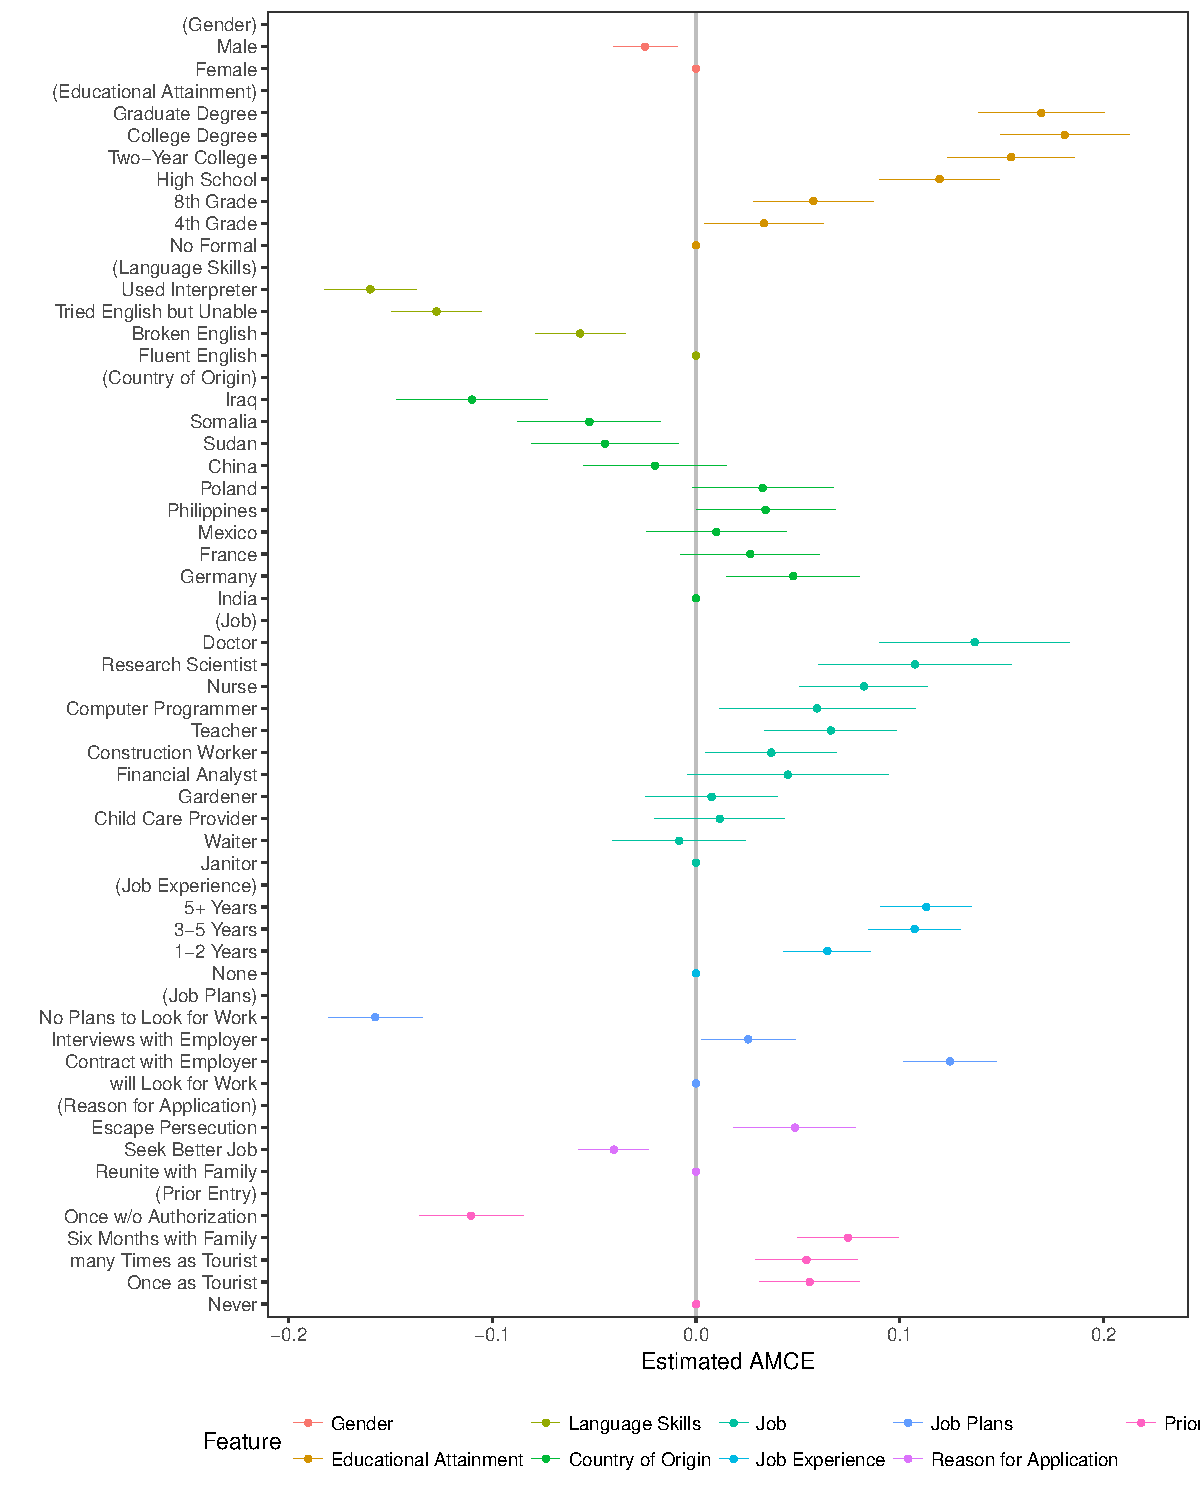
\includegraphics[width=\maxwidth]{figure/r_hainmueller_immigration-1} 

\end{knitrout}

\clearpage



\section{Arbitrary reference category choice}

\begin{knitrout}
\definecolor{shadecolor}{rgb}{0.969, 0.969, 0.969}\color{fgcolor}
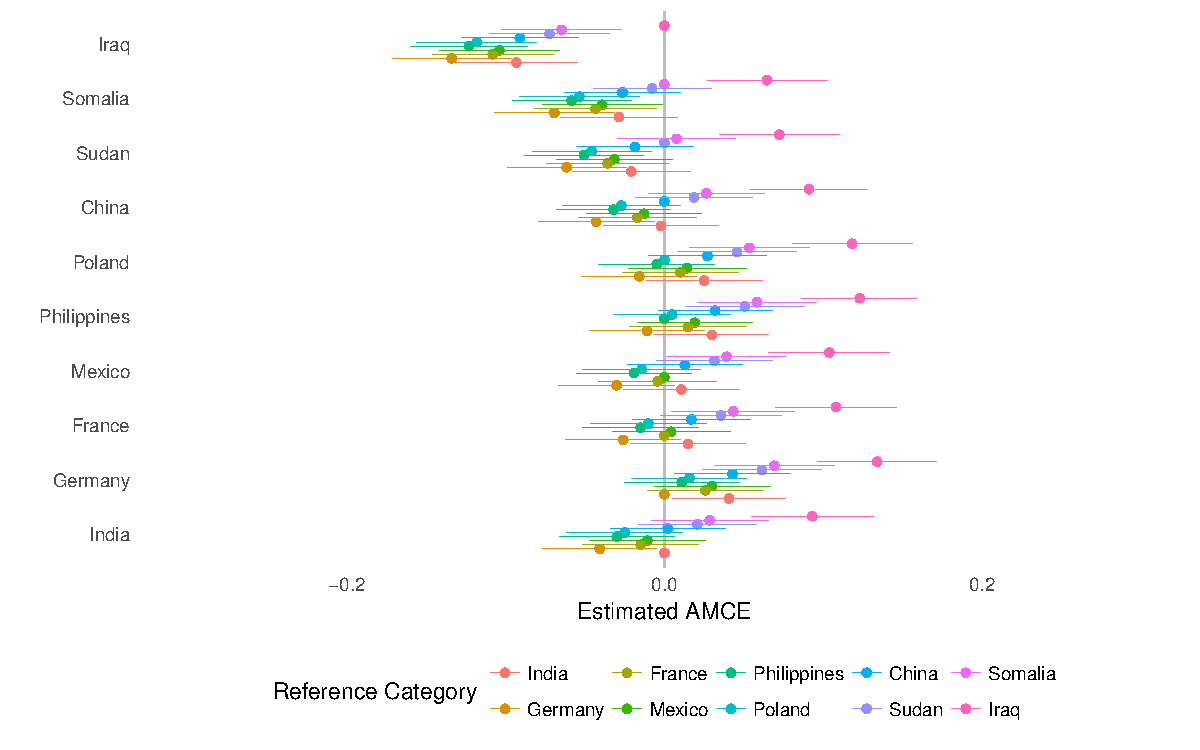
\includegraphics[width=\maxwidth]{figure/r_reference_category-1} 

\end{knitrout}

\begin{knitrout}
\definecolor{shadecolor}{rgb}{0.969, 0.969, 0.969}\color{fgcolor}
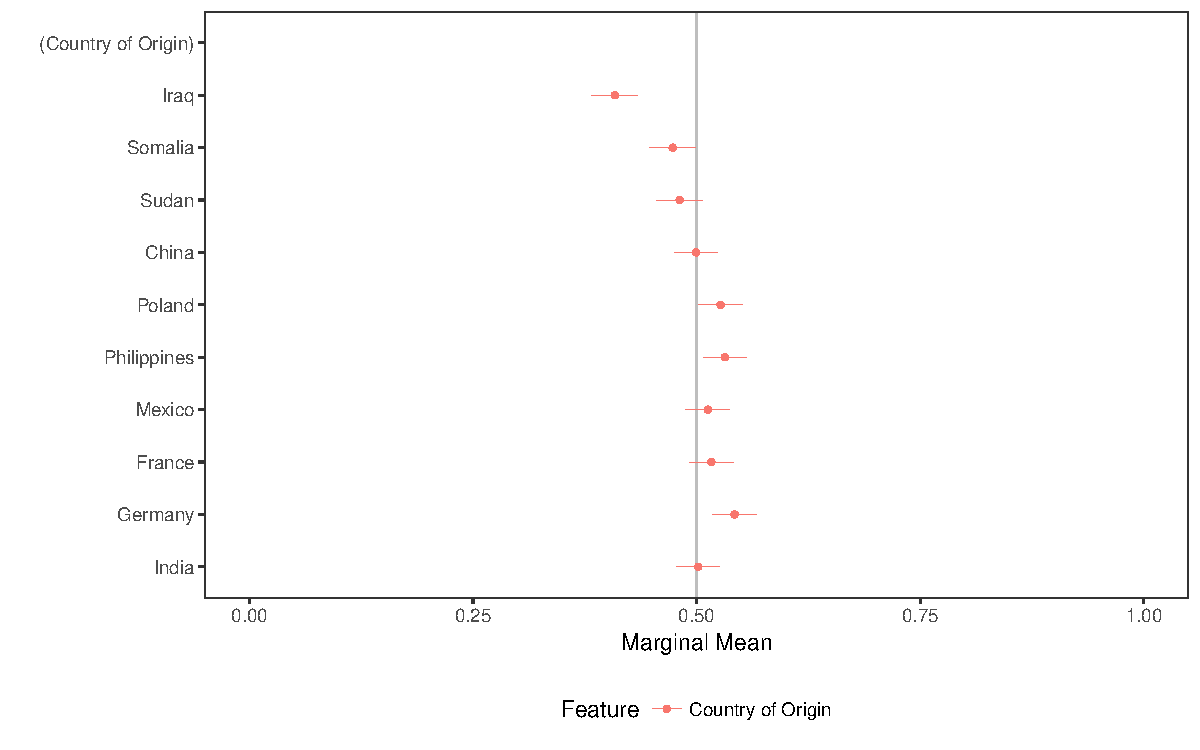
\includegraphics[width=\maxwidth]{figure/r_marginal_means-1} 

\end{knitrout}

\clearpage

\section{Subgroup Analysis}

A conventional presentation of subgroup analyses in a conjoint design is as follows. Note how the conditional AMCEs for several levels - Somalia, Sudan, China, Mexico, and France - flip signs. Yet the largest differences in preferences between the two groups are for Germany, France, Poland, and Somalia. Apparently similar patterns of AMCE mask where and in what direction preferences for the two subgroups differ.

\begin{knitrout}
\definecolor{shadecolor}{rgb}{0.969, 0.969, 0.969}\color{fgcolor}
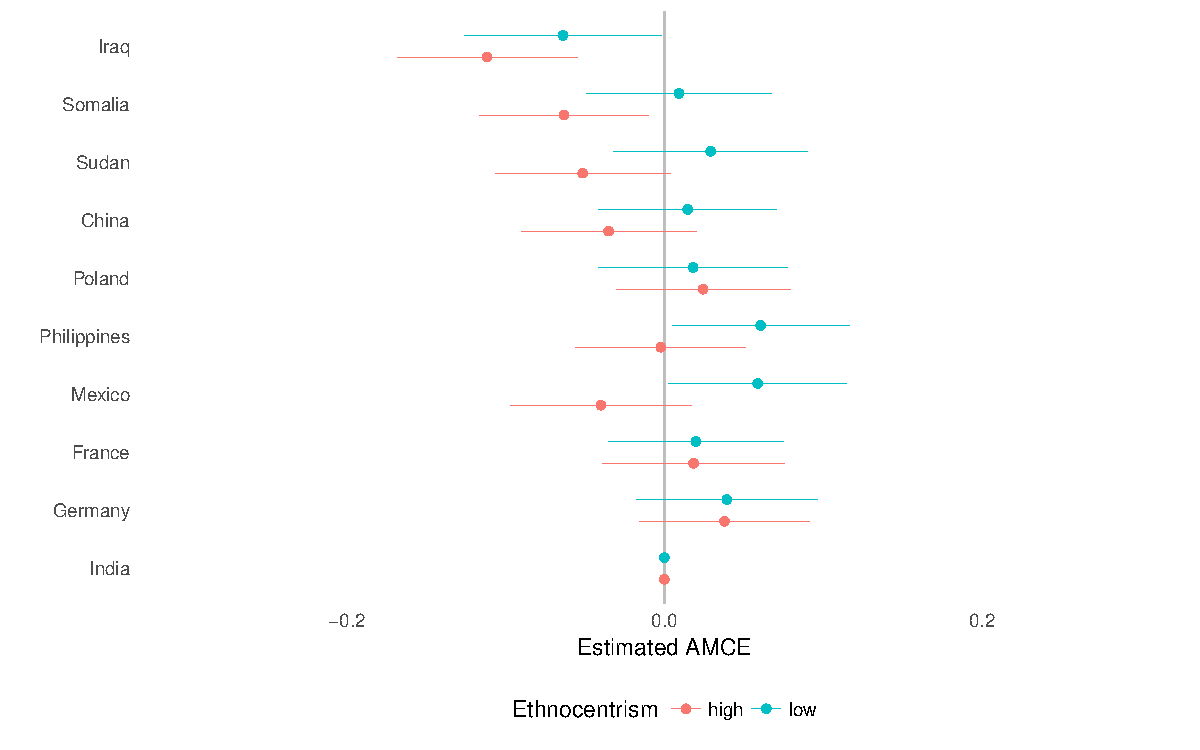
\includegraphics[width=\maxwidth]{figure/r_subgroup_results_amce-1} 

\end{knitrout}

\begin{knitrout}
\definecolor{shadecolor}{rgb}{0.969, 0.969, 0.969}\color{fgcolor}
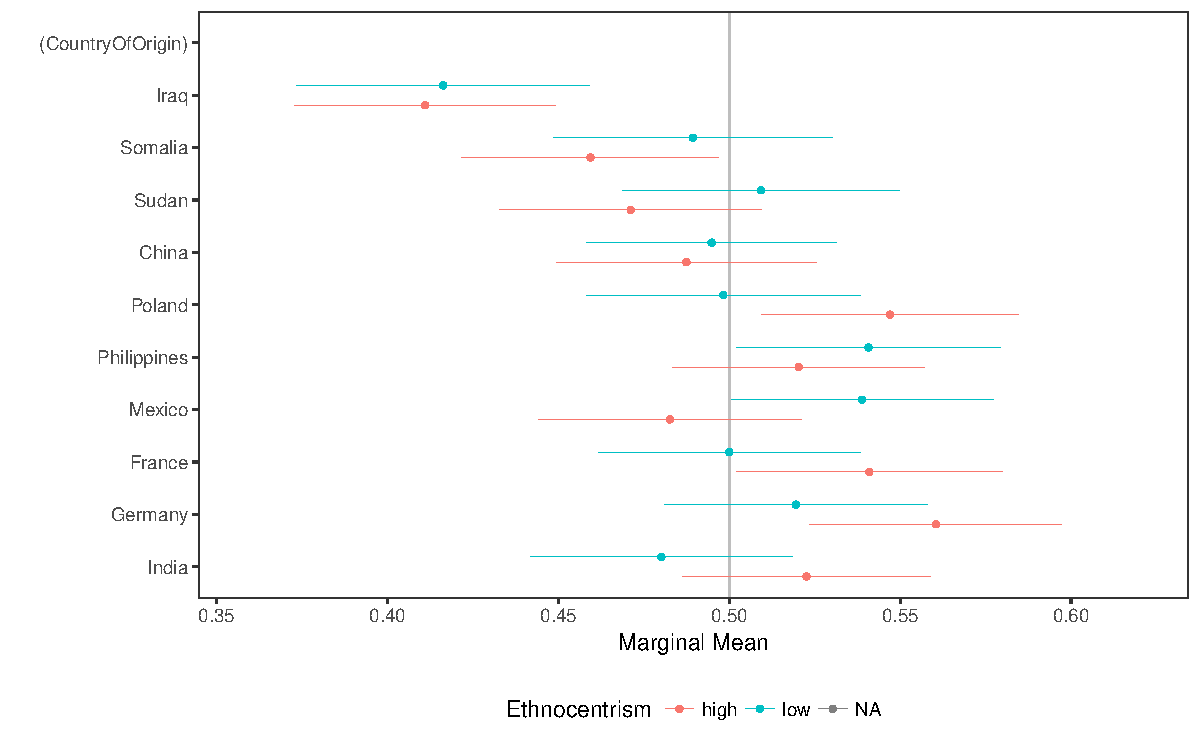
\includegraphics[width=\maxwidth]{figure/r_subgroup_marginal_means-1} 

\end{knitrout}

As we can see, however, while the difference in marginal means conveys the fixed difference in preferences between the two groups, the apparent difference in preferences between groups conveyed by a difference-in-AMCEs is sensitive to the reference category chosen when estimating the effects:

\clearpage

\begin{knitrout}
\definecolor{shadecolor}{rgb}{0.969, 0.969, 0.969}\color{fgcolor}
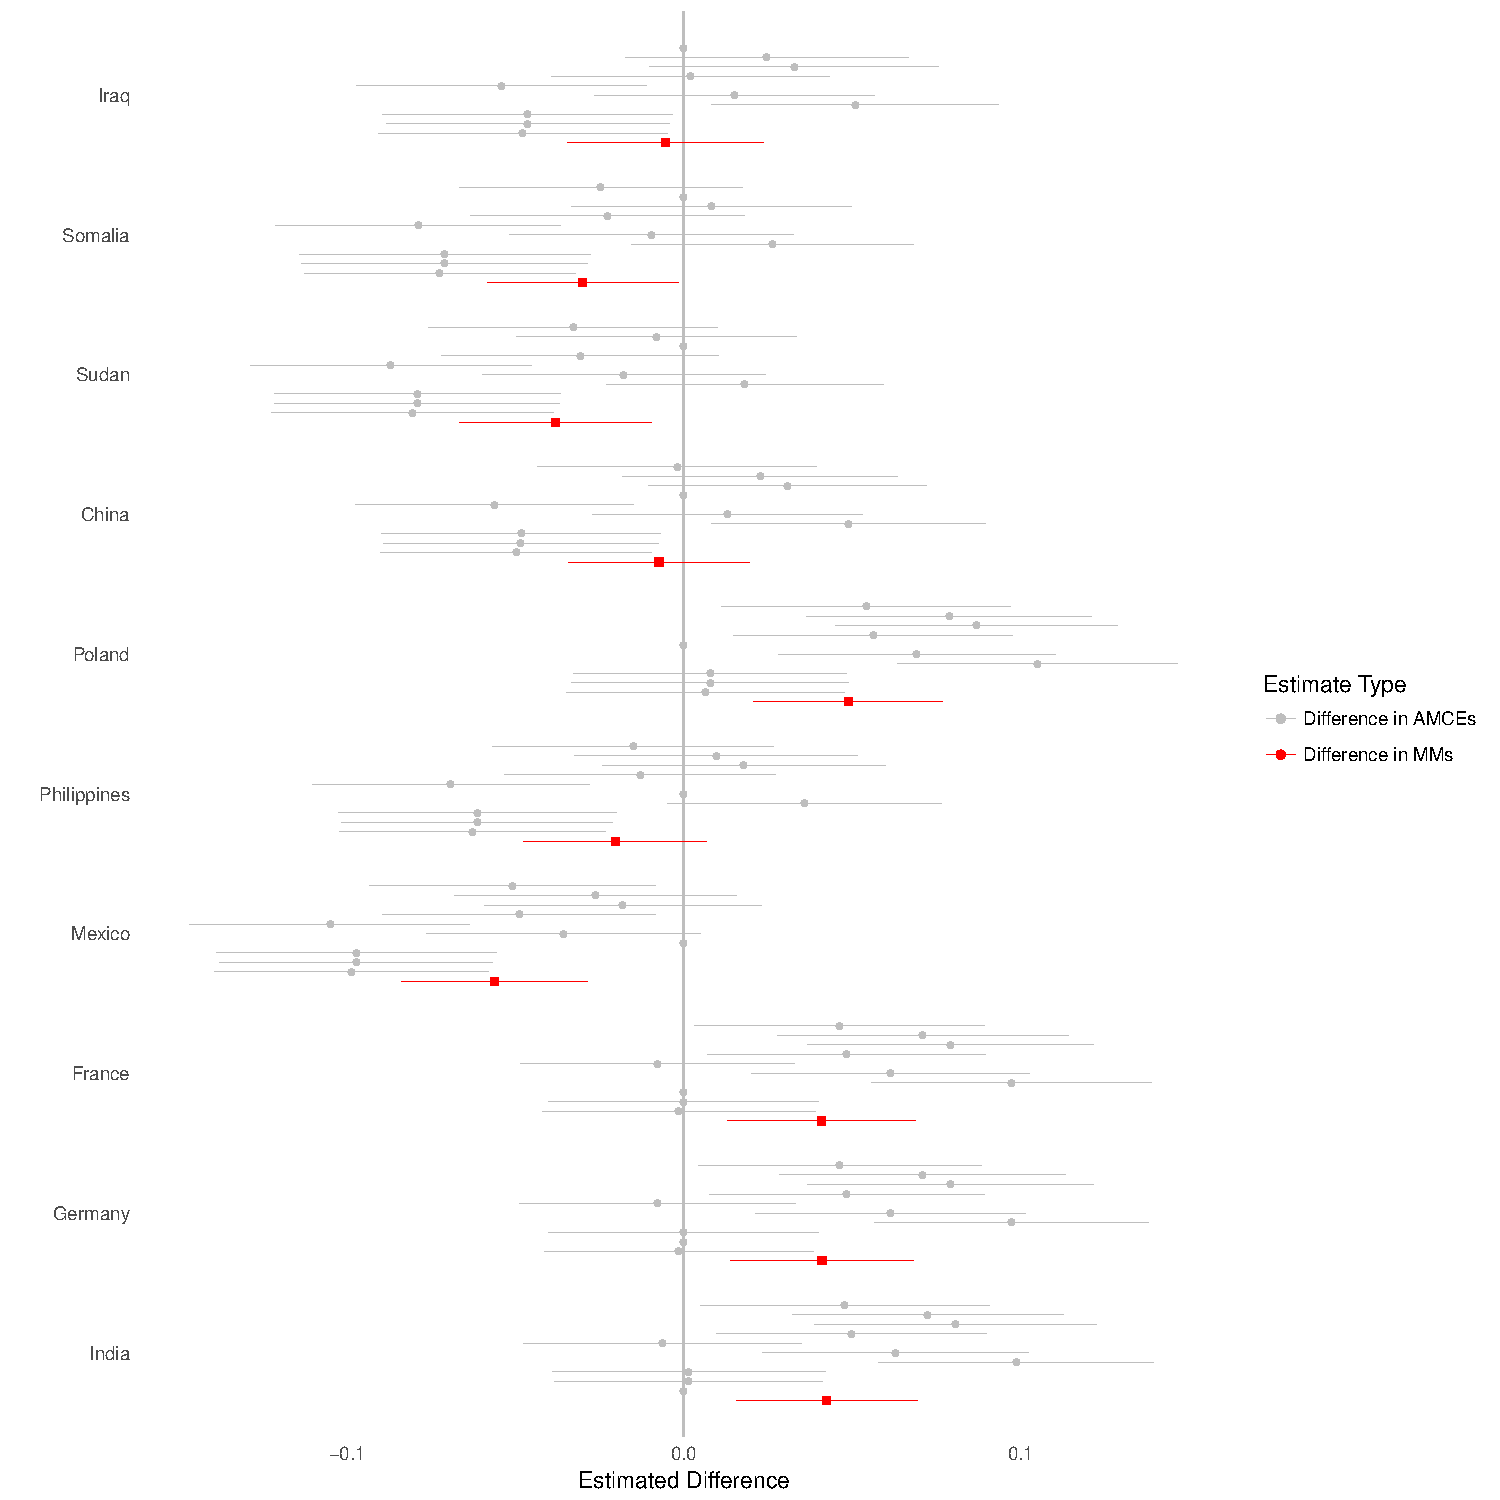
\includegraphics[width=\maxwidth]{figure/r_subgroup_results_mm-1} 

\end{knitrout}

Indeed, the difference in AMCEs most closely approximates the difference in marginal means (and thus the descriptive difference in preferences) when the true difference in preferences in the reference category is close to zero. For example, in the above figure differences in AMCEs are shown in gray and differences in marginal means are shown in red, for respondents scoring above-median (high) and below-median (low) in ethnocentrism for each possible country of origin in Hainmueller et al.'s (2014) immigration experiment. The difference in marginal means between high and low ethnocentrism respondents is smallest for immigrants arriving from Iraq. When Iraq is used as the reference category, the AMCE of Iraq is fixed at zero and the between-group difference in AMCEs is thus, by definition, also fixed at zero. These estimates are shown at the top of each grouping - as should be readily clear, when Iraq is used as the reference category, the difference in AMCEs for each of the other possible origin countries closely approximates (but does not exactly equal) the difference in marginal means for that origin country. Were there no feature level for which the two groups held similar preferences, then there would be no reference category that would generate differences in AMCES that were close to the difference in underlying marginal means.

When other origin countries are used as the reference category (wherein the underlying difference in preferences between high ethnocentrism and low enthnocentrism respondents is greater), then the difference in AMCEs provides biased estimates of the difference in preferences. Take, for example, the difference in preferences over immigrants from China, where high ethnocentrism respondents are less favourable to these immigrants than low ethnocentrism respondents. The difference in marginal means is -0.033. Yet differences in AMCEs for Chinese immigrants vary substantially depending on which other category is chosen as the baseline. If China is the baseline, the apparent difference in preferences is zero (definitionally). While in most cases the difference in AMCEs takes the same sign as the difference in marginal means, when either Mexico or Sudan is used as the reference category the apparent difference in preferences flips signs: high ethnocentrism respondents appear to be more rather than less favorable toward Chinese immigrants when the AMCEs are estimated in that way.

Yet the graph also makes clear that the differences in AMCEs all center upon the true difference in marginal means in a fixed manner.

Thus the choice of reference category - while seemingly irrelevant - has dramatic inferential consequences.

\section{Suggested Approaches}

% Present marginal means overall and for specific subgroups of interest


\section{Conclusion}

This paper has several identified challenges related to the analysis and reporting of conjoint experimental designs, particularly analyses of subgroup differences. It suggests that authors should report not only average marginal component effects (AMCEs) but also descriptive quantities that better convey subgroup differences.

\singlespacing
\bibliographystyle{apsa-leeper}
\bibliography{References}
\clearpage

\end{document}
